%!TEX root = ../dokumentation.tex
\chapter{Theory}

\section{Docker} 

To run applications on a cluster it is necessary to isolate these applications inside of a virtual container. Inside of these containers everything is available, what the application needs to get executed, but noting more. It is comparable to a \acs{VM} (\acl{VM}, but much more light weighted. This enables a very light deployment without unnecessary services or applications running in the background, which leads to a very performant execution.

%https://ieeexplore.ieee.org/abstract/document/7093032/

Docker is such a technology for virtualization of containers. It provides a industry-leading container engine technology with an easy way to build containers with a Dockerfile and manage and run those containers easily on your local device.

%https://www.docker.com/why-docker

The main difference between a container and a VM is the weight. While an average VM is hosting an operating system on top of a hypervisor on top of physical hardware. And on top of the OS of the VM the application is running. This affects the performance and the speed of the application in a very negative way, because a lot of unnecessary background proccesses are running. 

Docker solves this problem with a far more lightweight compute resource. The hypervisor of a docker container sits directly on the hosting operating system. This allows setting up several docker containers on only one phsyical machine and enables a high scalability. The differences between a VM and a docker container can be seen on the figure below.

%docker_container_infrastructure
%https://blog.mikesir87.io/2017/05/docker-is-not-a-hypervisor/

On the left side the infrastructure of a VM can be seen, on the right side the infrastructure of a Docker container. Both needs a physical defice infrastructure and the host operating system. On a VM on this Host Operating System a Hypervisor is running and on this Hypervisor several Guest OS can be running. On those again the apps itself can be executed and the necessary libraries and binaries are running.

In case of a docker container those binaries and libraries are directly running on the operating system without the need of a hypervisor or a complete version of a Guest OS. This also enables the app to be running on top of that. The containers are isolated from each other in different namespaces and own network stacks. This means, that processes running within a container cannot see or interact with processes of other containers and they don't get privileged access to sockets or interfaces of other containers.

%https://docs.docker.com/engine/security/security/

Additionally there is a Docker Daemon running in another process. The Docker Daemon has three main tasks - listening and processing API requests from the Docker client to run Docker commands, managing Docker objects (images, containers, volumes and networks) and parsing Dockerfiles for building docker images.

%file:///C:/Users/IBM_ADMIN/Downloads/20170830_thesis_final.pdf

Those Dockerfiles contains the definition of a basic image, on which the new container should be based on, and then every operation to be executed to build the container. This includes copying necessary files, installing underlying services, compilers and libraries, setting up the einvironment, executing the commands to start the app and more. All those operations creating a new layer in the container. This leads a container to look like can be seen in the figure 2.1.x below.

%docker layer image

This has the advantage, that similar containers, which has equal parts as other, already existing layers, can mount the existing layers from the other container and don't need to build every container for their own again. This makes the build of the docker containers much faster and the single images are smaller, which is especially a great gain for continious inntegration.

%https://tuhrig.de/layering-of-docker-images/

All in all Docker enables the creation of virtualized containers, in which applications can run isolated and independent from its environment. That's why it is a condition for deploying an application on a cluster, because there is no host operating system, on which the applications could be running otherwise.

%check?

\section{Kubernetes cluster solution}

One very common system for managing cluster systems as described in chapter 1.1 is \acl{K8s} - or short \acs{K8s}. Originally developed by Google and now maintained by the Cloud Native Computing Foundation, Kubernetes is an ``open-source platform for managing containerized workloads and services''.\textsuperscript{cmp.\cite{12}} For unterstanding what that means the concept of containers needs to be described first.

%https://kubernetes.io/docs/concepts/overview/what-is-kubernetes/

Containers are isolated, stand-alone packages of software, similar to processes. In those packages everything is included, which this piece of software needs, like runtime, libraries, settings and other system tools.  These containers have a completely different environment within themselves than outside. This environment includes for example network routes, dns settings and control group limits. This enables the possibility to share common resources and still be isolated from any other process as well as the host system. Thereby containers are always working the same, no matter on what system they run or in which environment.\textsuperscript{cmp.\cite{13}, \cite{14}}

%1 https://www.informatik-aktuell.de/entwicklung/methoden/kubernetes-architektur-und-einsatz-einfuehrung-mit-beispielen.html
%https://www.docker.com/what-container

Kubernetes is for an automating deployment, scaling and management of these containers within a cluster of nodes. Thereby a cluster consists of at least one master node and any number of worker nodes. Figure 2.1.1 shows the different services owned by master and worker nodes.

\begin{figure}[h]
\centering
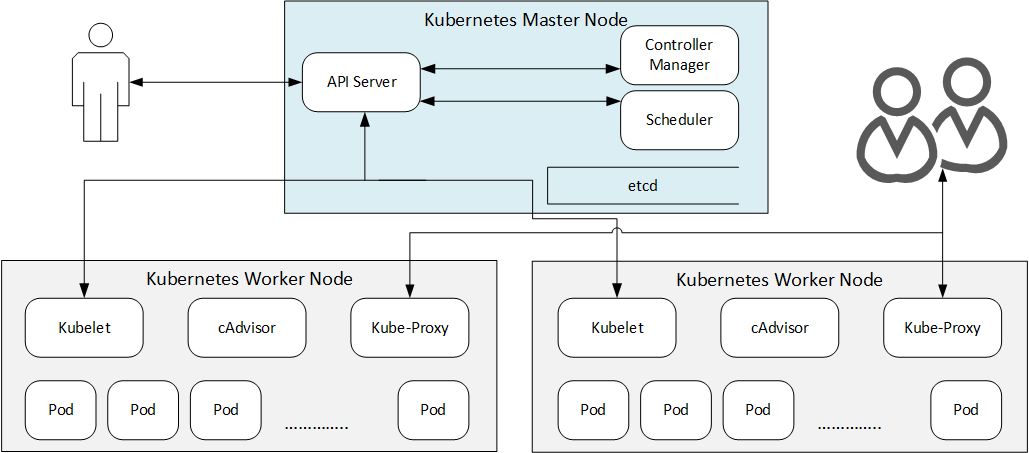
\includegraphics[width=\textwidth/5*3]{images/kubernetes_service_allocation.png}

\textsuperscript{Figure 2.1.1 Kubernetes allocation of services}\\
\textsuperscript{Based on retrieved information from \cite{13}}
\end{figure}

First there are several pods on each worker node. Pods are the smallest unit in Kubernetes. They contain one or more containers, which are deployed together on the same host. Thereby they can work together to perform a set of tasks.\textsuperscript{cmp.\cite{15}}%more?
%https://coreos.com/kubernetes/docs/latest/pods.html

On the master node there are an \acs{API} (\acl{API}) Server, a Controller Manager, a Scheduler and a key-value store called etcd.\textsuperscript{cmp.\cite{13}, \cite{16}}

The API Server is for clients to run their requests against. That means the API Server is responsible for the communication between Master and Worker nodes and for updating corresponding objects in the etcd. Also the authentication and authorization is task of the API Server. The protocol for the communication is written in \acs{REST} (\acl{REST}). For reacting on changes of clients there is also a watch mechanism implemented, which triggers an action after some specific changes, like the scheduler creating a new pod. This workflow is showed in figure 2.1.2.\textsuperscript{cmp.\cite{13}, \cite{16}}

\begin{figure}[h]
\centering
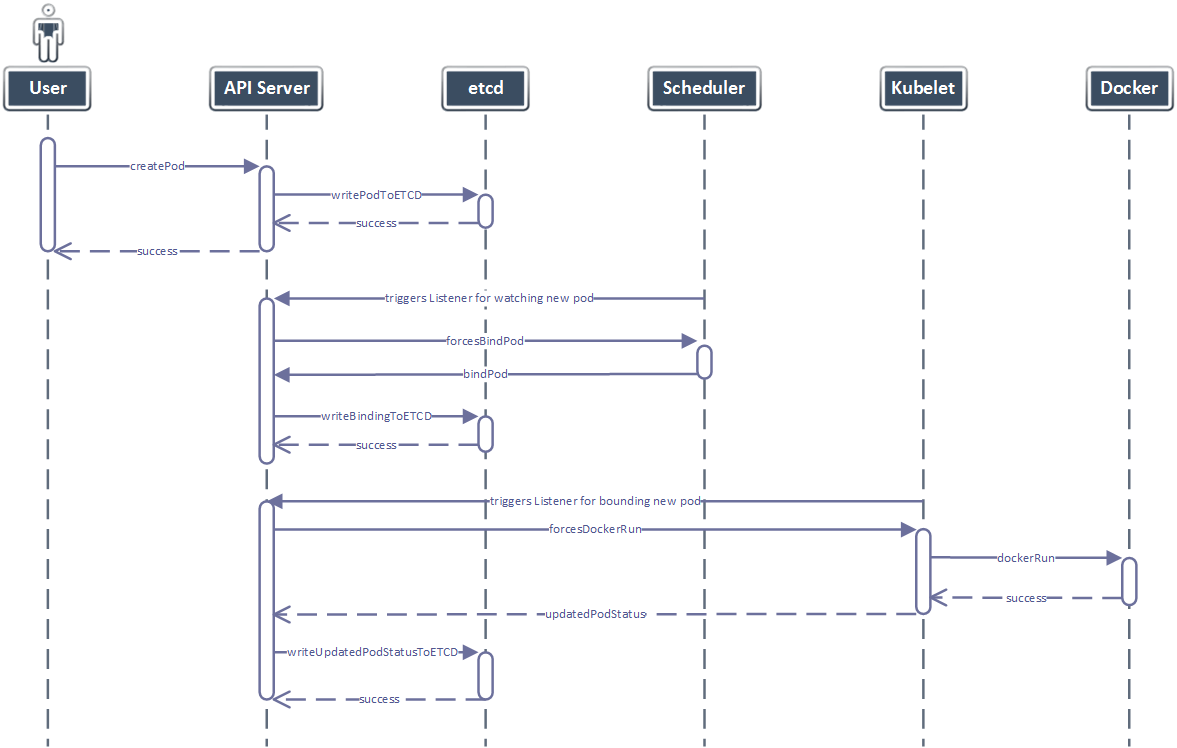
\includegraphics[width=\textwidth]{images/kubernetes_watcher_sequence.png}

\textsuperscript{Figure 2.1.2 Kubernetes API Server watcher sequence diagram}\\
\textsuperscript{Based on retrieved information from \cite{16}}
\end{figure}

There you can see the user creating a pod through a belonging request to the API Server. The API Server writes this change to the etcd. Afterwards the API Server recognizes a new pod in the etcd and invokes the Scheduler to create this new pod. What is the exact task of the scheduler is described later. After successfully creating and binding the new pod, the API Server writes this change to the etcd. Because of this change within the etcd the API Server invokes the kubelet, which is also described later in this chapter, of the corresponding node. This kubelet starts docker to create the containers of the pod. Kubelet responses with the new status of the pod, which is then written to the etcd by the API Server. After that the creation of the new pod is successfully finished.\textsuperscript{cmp.\cite{13}, \cite{16}}

The Controller Manager is a daemon, which embeds all of the Kubernetes controller. Examples for them are the Replication Controller or the Endpoint Controller. Those controllers are watching the state of the cluster through the API Server. Whenever a specific action happens, it performs the necessary actions to hold the current state or to move the cluster towards the desired state. For providing an example: If the Replication Controller recognizes, that one replication of a pod has been destroyed for some reason, it will take care of triggering the creation of a new replication.\textsuperscript{cmp.\cite{13}, \cite{16}}

The scheduler manages the binding of pods to nodes. Therefore it watches for new deployments as well as for old ones to create new pods if a new deployment is created or recreating a pod whenever a pod gets destroyed. The scheduler organizes the allocation of the pods within the cluster on the basis of available ressources of the pods. That means, that it always create pods, where the most resources are available, or reorganize the allocation if there is a change in the resource allocation of the cluster.\textsuperscript{cmp.\cite{13}, \cite{16}}%??

Figure 2.1.3 shows the way the Scheduler works, when new nodes are connected. As long as there are only two nodes and four pods need to be deployed, it allocates those four pods to the two nodes . As soon as there are more nodes connected, the scheduler recognizes free resources and reallocate the pods to these new nodes.

\begin{figure}[h]
\centering
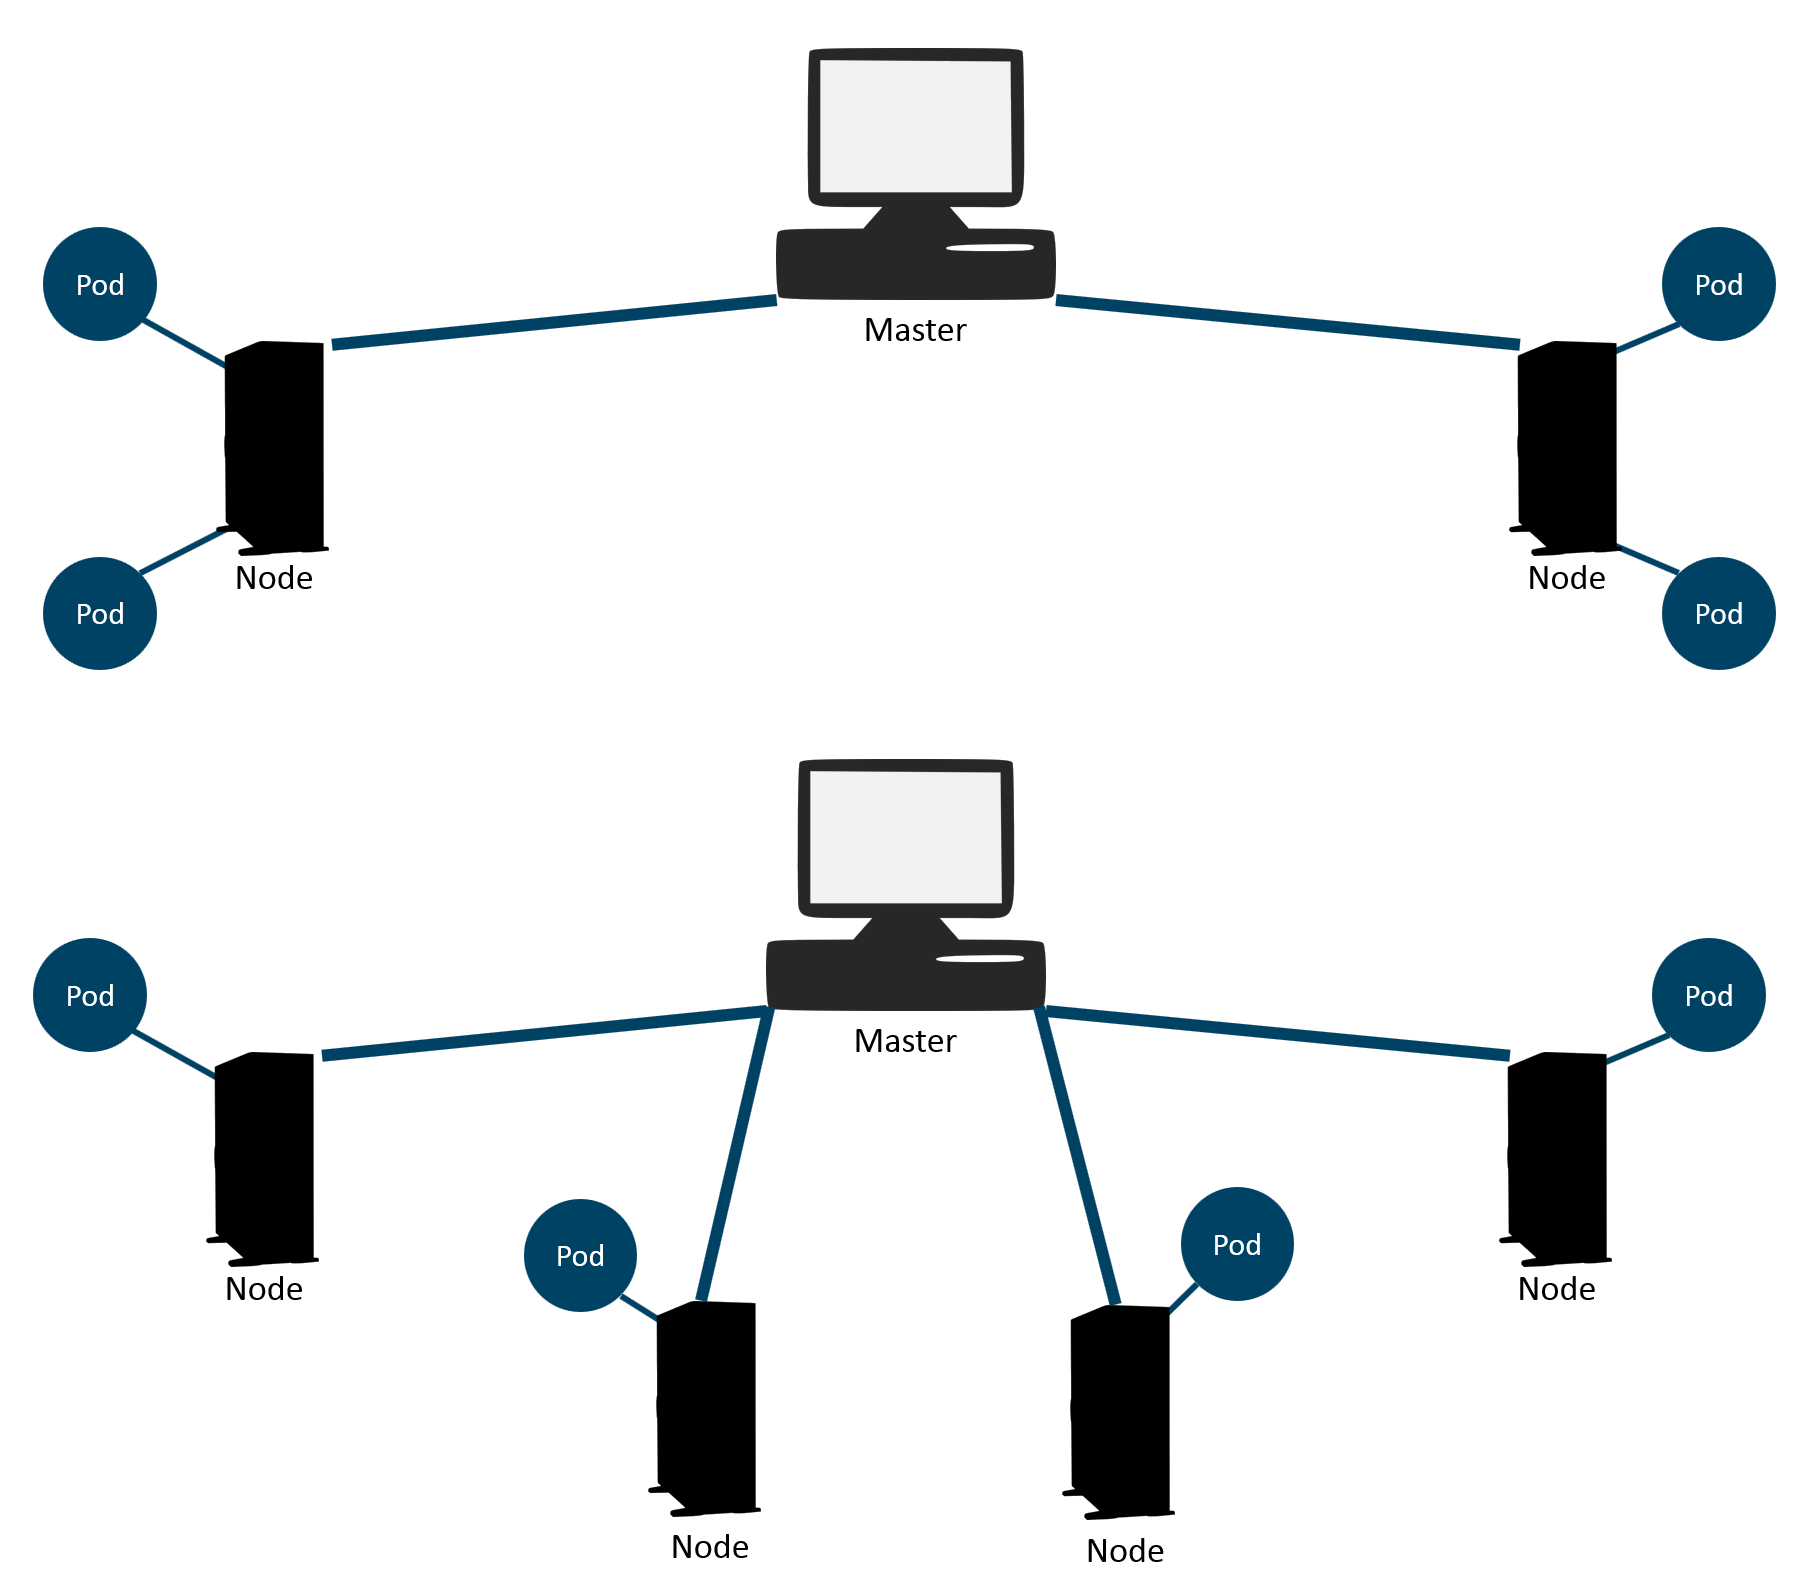
\includegraphics[width=\textwidth/5*3]{images/kubernetes_scheduler.png}

\textsuperscript{Figure 2.1.3 Kubernetes API Server watcher sequence diagram} \\
\textsuperscript{Based on retrieved information from \cite{17}}
\end{figure}
%https://www.informatik-aktuell.de/fileadmin/_processed_/b/6/csm_K8s_abb1_fricke_b5ce6bd912.png

The etcd is a key-value store, which stores the configuration data and the condition of the Kubernetes cluster. The etcd also contains a watch feature, which listens to changes to keys and triggers the API server to perform all necessary actions to move the current state of the cluster towards the desired state.\textsuperscript{cmp.\cite{13}, \cite{16}}

The worker node consists of a Kubelet, a cAdvisor, a Kube-Proxy and - as mentioned before - several Pods. 

The kubelet needs to be used if a new pod should be deployed. Then it gets the action to create all needed containers. For that it uses Docker to create them. Afterwards it combines some containers into one pod. Conainers in one pod are always started and stopped together. This pod will then be deployed on the node, on which the kubelet is located.\textsuperscript{cmp.\cite{13}, \cite{16}}

The cAdvisor measures the usage of CPU-resources as well as demanded memory on the node, on which it is located, and notifies the master about it. Based on those measurements the scheduler allocates the pods within the cluster to ensure the best possible allocation of resources.\textsuperscript{cmp.\cite{13}, \cite{16}}

The kube-proxy is a daemon, that runs as a simple network proxy to provide the possibility of communicating to that node within the cluster. Additionally it runs a load balancer for the services on that node.\textsuperscript{cmp.\cite{13}, \cite{16}}

Through this architecture Kubernetes enables different possibilities to deploy pods within the cluster. The simplest one is to deploy a specific pod directly through the 
\begin{lstlisting}[caption={Create Kubernetes pod},captionpos=b]
kubectl create -f `image\_path'
\end{lstlisting}
command. This deploys the pod described in the file, but it doesn't ensure the failure safety. That means if the pod gets destroyed for some reason, no matter if it has been destroyed by accident or intended, it won't be recreated and deployed again automatically. 

%1
%2 https://medium.com/jorgeacetozi/kubernetes-master-components-etcd-api-server-controller-manager-and-scheduler-3a0179fc8186

Another possibility is to create a deployment. Therefore the image has to be embedded within a replicaset and this replicaset within a deployment. If this deployment is created, it will automatically create every pod of the replicaset. If one pod gets terminated, no matter if manually or because of an error, it will be directly recreated and deployed.\textsuperscript{cmp.\cite{13}, \cite{18}}

This procedure also enables the possibility to execute dynamical rolling updates. If you execute the command
\begin{lstlisting}[caption={Create Kubernetes deployment},captionpos=b]
kubectl set image deployment/name-deployment name=name:1.1.1
\end{lstlisting}
Kubernetes will start a Rolling Update. This causes the creation of a new replicaset, which uses pods of the new version. While the new replicaset will be scaled up, the old one will be scaled down step by step. This enables the maintenance of a deployment even while an update is enrolled, so that the users can still use the services while those are updating. That means, that there is never a need of a system to shut down because of an update, which needs to be enrolled, and the system guarantees its high availability.\textsuperscript{cmp.\cite{13}, \cite{18}}

A third possibility to deploy pods are services. Services are used to enable the usage of pods from outside the cluster. Therefore it gets the pod from the targetPort of the belonging node and creates a random port on this node. This port serves as endpoint for the LoadBalancer. Through this, everybody can now communicate with this pod.\textsuperscript{cmp.\cite{13}, \cite{18}}

This is how Kubernetes ensures High Availability as well as Load Balancing at the same time. Through the possibility of replicate every pod several times it is ensured that whenever one pod fails for some reason, another is already prepared to help out and take over the job. Even the master can and should be replicated to ensure a functional system, even if one master has been destroyed. For production environment it's recommended to have 3, 5 or 7 master nodes running at the same time. For facilitating the High Availability almost every unit of a Kubernetes cluster is stateless and could be run redundant in several instances. Only the etcd key value store is stateful. For solving that problem in case of failure of the node, which owns the etcd, there is a leader election between all master node replicas to determine the new leading etcd.\textsuperscript{cmp.\cite{13}, \cite{18}}

%1
%2
%https://deis.com/blog/2016/kubernetes-overview-pt-1/

All in all Kubernetes combines all the benefits of cluster applications in one software. High availability as well as load balancing is guaranteed and it also ensures a high scalability, rolling updates and auto-scaling. Compared to other cluster systems, like Docker swarm, it has the biggest community and it can support clusters of up to 5000 nodes, which enables using Kubernetes even for very big clusters. For example the whole Google Cloud System runs on a Kubernetes cluster. Performing tests of Kubernetes shows, that in 99\% the API responses in less than one second and also their pods start in less than five seconds in 99\% when starting containers with pre pulled images. This all makes Kubernetes maybe one of the most flexible and fastest cluster systems. In exchange for that flexibility it is more difficult to set it up, because you have to do it all on your own. But only that way it can be ensured, that it runs fast and flexible in the same time, which is the reason for Kubernetes being so popular.\textsuperscript{cmp.\cite{19}, \cite{20}}

%https://platform9.com/blog/kubernetes-docker-swarm-compared
%https://www.redhat.com/de/topics/containers/what-is-kubernetes ???

\section{Apache Kafka}

\section{Open Source Routing Machine}

\section{Mongo Database}

\section{DRL Car Sharing Service}

%\section{CPLEX}